\documentclass[a4paper,11pt]{scrartcl}
\usepackage{hyperref}
\usepackage{amsmath}
\usepackage{amsfonts}
\usepackage{amssymb}
\usepackage{amsbsy}
\usepackage{bm}
\usepackage{graphicx}
\usepackage{extarrows}

\newcommand{\ie}{i.\,e.}%
\newcommand{\eg}{e.\,g.}%
\newcommand{\etal}{et\,al.}%
\newcommand{\wrt}{w.r.t.}%
\newcommand{\sign}{\operatorname{sign}}

\newcommand{\leviCivita}{\varepsilon}

% comma and period at end of formulas
\newcommand{\formComma}{\,\text{,}}
\newcommand{\formPeriod}{\,\text{.}}

% real and complex numbers
\newcommand{\R}{\mathbb{R}}%
% \newcommand{\C}{\mathbb{C}}%

% bold symbols
\newcommand{\xb}{\mathbf{x}}%
\newcommand{\rb}{\mathbf{r}}%
\newcommand{\ub}{\mathbf{u}}%
\newcommand{\nb}{\mathbf{n}}%
\newcommand{\eb}{\bm{e}}%
\newcommand{\gb}{\mathbf{g}}%
\newcommand{\Xb}{\mathbf{x}}% parametrization X:{(theta,phi)} --> R3

\newcommand{\alphab}{\bm{\alpha}}% for \pb^{\flat}
\newcommand{\betab}{\bm{\beta}}% for \qb^{\flat}

\newcommand{\eqAngle}{\phi}

% director and its components
\newcommand{\pb}{\mathbf{p}}%
\newcommand{\p}{\textup{p}}%
% test funciton and its components
\newcommand{\q}{\textup{q}}%
\newcommand{\qb}{\mathbf{q}}%
\newcommand{\tb}{\mathbf{t}}%
\newcommand{\Eb}{\mathbf{E}}%
\newcommand{\Mbb}{\mathbf{M}}%
\renewcommand{\sb}{\mathbf{s}}%
\newcommand{\vb}{\mathbf{q}}%to unify test functions

\newcommand{\alphav}{\underline{\bm{\alpha}}} % for vector-1-forms, like PD-1-form
\newcommand{\betav}{\underline{\bm{\beta}}} % for vector-1-forms, like PD-1-form

\newcommand{\abs}[1]{\lvert#1\rvert}%
\newcommand{\norm}[1]{\lVert#1\rVert}%
\newcommand{\scalarprod}[1]{\big\langle{#1}\big\rangle}%
\newcommand{\Scalarprod}[1]{\left\langle{#1}\right\rangle}%

% derivatives
\newcommand{\dif}{\textup{d}}
\newcommand{\exd}{\mathbf{d}} %exterior derivative
\newcommand{\ds}{\,\dif{s}}
\newcommand{\dr}{\,\dif\rb}
\newcommand{\dx}{\,\dif\xb}
\newcommand{\dxhat}{\,\dif\hat{\xb}}
\newcommand{\dt}{\partial_t}

% differential forms for integration
\newcommand{\dS}{\,\dif{\surf}}
\newcommand{\dV}{\,\dif{V}}

% functional derivative
\newcommand{\fdif}{\operatorname{\delta}\!}
\newcommand{\Fdif}[2]{\frac{\fdif{#1}}{\fdif{#2}}}% dF / du	
\newcommand{\FFdif}[3]{\frac{\fdif^2{#1}}{\fdif{#2}\fdif{#3}}}% d^2F / dudv	

\newcommand{\FF}{\mathrm{F}}
\newcommand{\F}[1]{\FF_\mathrm{#1}}

% surface and domain
\newcommand{\Sp}{\mathbb{S}^2}
\newcommand{\ellipsoid}{\mathcal{E}}
\newcommand{\surf}{\mathcal{S}}
\newcommand{\domain}{\Omega}

\newcommand{\meanCurvature}{\mathcal{H}}
\newcommand{\gaussianCurvature}{\kappa}

% surface (differential operators)
\newcommand{\Grad}{\operatorname{Grad}}
\renewcommand{\div}{\operatorname{div}}%
\newcommand{\Rot}{\operatorname{Rot}}%
\newcommand{\rot}{\operatorname{rot}}%
\newcommand{\DivSurf}{\Div_{\surf}}%
\newcommand{\GradSurf}{\Grad_{\surf}}
\newcommand{\laplace}{\Delta}
\newcommand{\laplaceBeltrami}{\Delta_{\surf}}
\newcommand{\vecLaplace}{\boldsymbol{\Delta}}
%\newcommand{\laplaceDeRahm}{\vecLaplace^{\textup{dR}}_{\surf}}
\newcommand{\laplaceDeRham}{\vecLaplace^{\textup{dR}}}
\newcommand{\laplaceDeRahm}{\laplaceDeRham}
\newcommand{\laplaceRotRot}{\vecLaplace^{\textup{RR}}}
\newcommand{\laplaceGradDiv}{\vecLaplace^{\textup{GD}}}

\newcommand{\laplaceDeRhamTilde}{\widehat{\vecLaplace}^{\textup{dR}}}
\newcommand{\NablaSurf}{\nabla_{\surf}}
\newcommand{\gDerivative}{D}

\newcommand{\laplaceDeRhamDiffuse}{\widehat{\vecLaplace}^{\textup{dR}}_{\phi}}

\newcommand{\surfNormal}{\boldsymbol{\nu}}
\newcommand{\surfNormalI}{\nu}

\newcommand{\ProjectSurf}{\pi_\surf}

\newcommand{\Tangent}{\mathsf{T}}

% General
\newcommand{\vect}[1]{\mathbf{#1}}
\newcommand{\tensor}[1]{\mathbf{#1}}

\newcommand{\Span}[1]{\operatorname{Span}\!\left\{ #1 \right\}}

\newcommand{\AMDIS}{\texttt{AMDiS}}
\newcommand{\PETSC}{\texttt{PETSc}}

% Constants
\newcommand{\K}{{K}} % one-constant
\newcommand{\Ki}{{K_1}} % frank-constant K1
\newcommand{\Kii}{{K_2}} % frank-constant K2
\newcommand{\Kiii}{{K_3}} % frank-constant K3
\newcommand{\Kn}{{\omega_n}} % penalty constant for normality
\newcommand{\Kt}{{\omega_t}} % penalty constant for tangentiality

% Energies
\newcommand{\EF}{E^{\textup{F}}} % 3D Frank-Energy
\newcommand{\EFSurf}{E^{\textup{F}}_{\surf}} % Frank-Energy on surface
\newcommand{\ESurf}{E_{\surf}} % intrinsic Frank-Energy plus normalizing term on surface

\newcommand{\EE}{\F{\omega}^\surf}
\newcommand{\E}[1]{\EE[#1]}


\newcommand{\Ltwo}[2]{L^2( #1;\, #2)}%
\newcommand{\LS}{L^2(\surf)}%
\newcommand{\LtwoProd}[1]{\big({#1}\big)_{\LS}}%

\newcommand{\C}[2]{{C}( #1;\, #2)}
\newcommand{\Csurf}[1]{{C}^{#1}(\surf)}
\newcommand{\Cdomain}[1]{{C}^{#1}(\domain)}
\newcommand{\extend}[1]{\widehat{#1}}

\newcommand{\Hdr}[2]{H^{\textup{DR}}( #1;\, #2)} %
\newcommand{\HdrExt}[2]{H^{\textup{DR}}( #1;\, #2)} % \extend{H}^{\textup{DR}}\left( #1 ; #2 \right)
\newcommand{\HdrDiffuse}[2]{H^{\textup{DR}}( #1;\, #2)} %\extend{H}^{\textup{DR}}_{\phi}\left( #1 ; #2 \right)

\newcommand{\Hi}[1]{H^{1}(#1)}

\newcommand{\pExt}{\extend{\pb}}
\newcommand{\qExt}{\extend{\qb}}
\newcommand{\nExt}{\extend{\surfNormal}}

% rotation angle
\newcommand{\rotAngle}{\psi}

% DEC declarations
\newcommand{\SC}{\mathcal{K}} % simplicial complex
\newcommand{\Vs}{\mathcal{V}} % set of vertices
\newcommand{\Es}{\mathcal{E}} % set of edges
\newcommand{\Fs}{\mathcal{T}} % set of faces
\newcommand{\face}{T} % one face
\newcommand{\FormSpace}{\Lambda^{1}} % space of 1 forms
\newcommand{\PDT}{\mathfrak{T}} % PD-Tangential-Space

% for commends among each other
\newcommand{\simon}[1]{{\color{red}#1}}
\newcommand{\ingo}[1]{{\color{blue}#1}}
\newcommand{\micha}[1]{{\color{green}#1}}

\newcommand{\hidden}[1]{}

%\theoremstyle{plain}
\newtheorem{lem}{Lemma}
\newtheorem{thm}{Theorem}
\newtheorem{prop}[thm]{Proposition}
\newtheorem{rem}{Remark}[section]
\newtheorem{exmp}{Example}[section]

%\theoremstyle{definition}
\newtheorem{defn}{Definition}

\makeatother
\providecommand*{\thmautorefname}{Theorem}
\providecommand*{\remautorefname}{Remark}
\providecommand*{\defnautorefname}{Definition}
\providecommand*{\algorithmautorefname}{Algorithm}
%\addto\extrasenglish{%
  %\renewcommand{\chapterautorefname}{Chapter}%
  %\renewcommand{\sectionautorefname}{Section}%
  %\renewcommand{\subsectionautorefname}{Section}%
  %\renewcommand{\subsubsectionautorefname}{Section}%
  %\renewcommand{\paragraphautorefname}{Section}%
%}
\newcommand*{\End}{\hfill\ensuremath{\vartriangleleft}}%
\newcommand*{\END}{\hfill\ensuremath{\blacktriangleleft}}%




% standard R3 basis
\newcommand{\EuBase}[1]{\eb^{#1}}
% surface parameter
\newcommand{\pstretch}{C}
\newcommand{\pprop}{r}
\newcommand{\ppress}{B}

\title{Notes On Nonic Surfaces Experiment} 

\begin{document}
\maketitle

\section{Surface Descriptions}
We are starting with the standard parametrization of the unit sphere \( \Sp \)
with local coordinates \(  \theta\in\left[ 0,\pi \right]\) and \( \phi\in\left[ 0,2\pi\right) \), i.e.,
\begin{align}
      \Xb_{\Sp}(\theta,\phi) &= 
                      \sin\theta\cos\phi\EuBase{x} +  \sin\theta\sin\phi \EuBase{y} + \cos\theta\EuBase{z} \formPeriod
\end{align}
For stretching the unit sphere by a displacement function \( f:[-1,1] \rightarrow \R \) in the \( x \)-direction depending on the \( z
\)-positions 
and pressing to the \( x \)-\( z \)-plane by a press factor \( \ppress\in [0,1) \),
we obtain the surface
\begin{align}
  \Xb_{f,\ppress}(\theta,\phi) &:= \Xb_{\Sp}(\theta,\phi) + f(\cos\theta)\EuBase{x} - B\sin\theta\sin\phi\EuBase{y}
\end{align}
and with \( \ppress\nearrow 1 \) the surface becomes flat.
We choose for the displacement function \( f \) a double well function,
which should break the symmetry referring to the \( x \)-\( y \)-plane,
so that the north pole (\( z=1 \)) of the initial sphere is shifting right in  \( x \)-direction by \( \pstretch>0 \)
and the south pole (\( z=-1 \)) by \( \pprop\cdot\pstretch  \) with the proportion factor \( 0 \le \pprop < 1 \).
This implies
\begin{align}
  f(z) &:= f_{\pstretch,\pprop}(z) = \frac{1}{4} \pstretch z^2 \left[(z+1)^2 (4-3 z)+\pprop (z-1)^2 (4+3 z)\right]
\end{align}
where the double well conditions \( f(1) = \pstretch \), \( f(-1)=\pprop\cdot\pstretch \) and \( f'(1)=f'(0)=f'(-1)=0 \) are fulfilled,
see for example \autoref{fig:SphereToNonicPressed}.
\begin{figure}
  \centering
  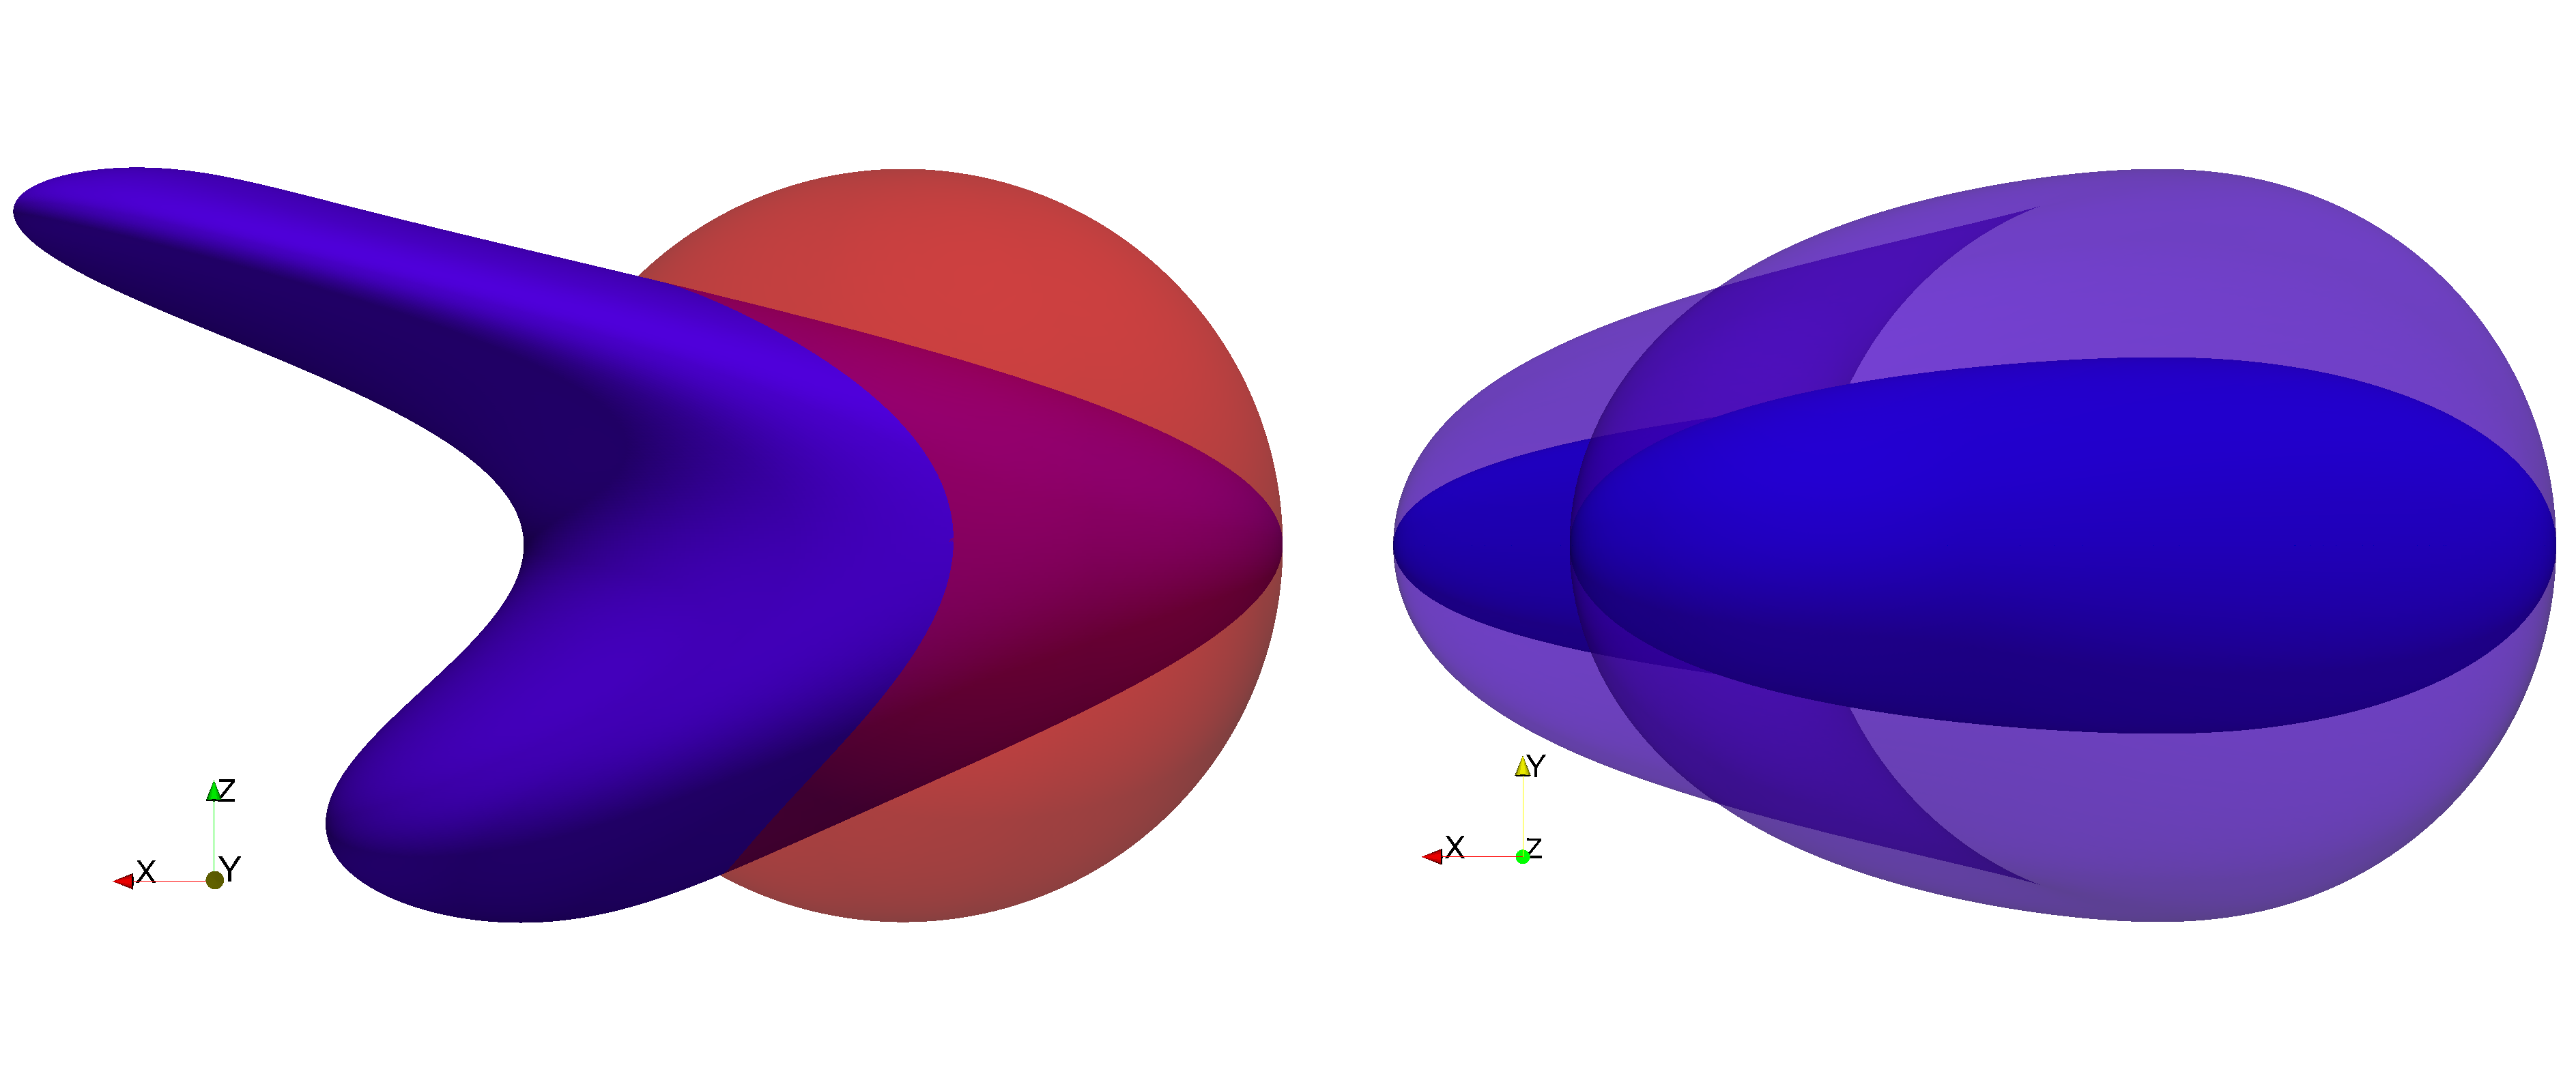
\includegraphics[width=.9\textwidth]{stuff/paraview/Sphere2Nonic2NonicPressed.png}
  \caption{Nonic Surface with parameters \( \pprop = 0.5 \), \( \pstretch = 2 \) and \( \ppress = 0.5 \).
           The left figure shows the stretching of the unit sphere in the \( x \)-direction.
           Hence, by the choice of the parameter, the north pole (\( z=1 \)) is shifting by \( \pstretch = 2 \) 
           and the south pole (\( z=-1 \)) by \( \pprop\cdot\pstretch = 1 \) units of length to the left. 
           The right figure shows the pressing of the resulting surface to the \( x \)-\( z \)-plane by the press factor \( \ppress=0.5 \).
           }
  \label{fig:SphereToNonicPressed}
\end{figure}
For the immersion \( \Xb_{\ppress,\pstretch,\pprop} := \Xb_{f,\ppress}:[0,\pi]\times[0,2\pi)\rightarrow\R^{3}  \)
the surface family \( \surf_{\ppress,\pstretch,\pprop} := \text{Im}(\Xb_{\ppress,\pstretch,\pprop})\)
can also expressed implicitly by the 0-Levelset of the function
\begin{align}
  \varphi_{\ppress,\pstretch,\pprop}(x,y,z) &:= \left( x - f_{\pstretch,\pprop}(z) \right)^{2} + \frac{1}{(1-\ppress)^{2}}y^{2} + z^{2} - 1
\end{align}
defined in a smooth neighbourhood of the surface.
We call \( \surf_{\ppress,\pstretch,\pprop} \) a \textbf{Nonic Surface}, because \( \varphi_{\ppress,\pstretch,\pprop} \) is a polynomial of
degree 10.
The gradient
\begin{align}
  \nabla\varphi_{\ppress,\pstretch,\pprop}(x,y,z) &= 2
      \begin{bmatrix}
        x - f_{\pstretch,\pprop}(z) \\
        \frac{y}{(1-\ppress)^{2}} \\
        z-(x-f_{\pstretch,\pprop}(z))f'_{\pstretch,\pprop}(z)
      \end{bmatrix}\formComma
\end{align}
restricted to the surface, points in the direction of the outer surface normals.

\section{Initial Solutions Construction for the Frank-Oseen-Equations}
To solve the director field evololutions in paper \textbf{NUMERICAL METHODS FOR ORIENTATIONAL ORDER ON SURFACES},
we have to assign initial fields \( \pb \), \( \alphab = \pb^{\flat} \) respectively,
with \( \|\pb\| = \|\alphab\| = 1 \) a.e..
\subsection{4 Defect Init}
The 4 defect configuration, 3 with positive charge at the bulges and 1 with negative charge at the saddle point, 
is potentially stable depending on the choice of the surface
parameter.
The proportion factor \( \pprop\in[0,1) \) prevent a metastable solution, because the resulting symmetry break induce different dynamics
for  2 defect locations on the bulges.
This implies, that the defect on the smaller bulge and the saddle point defect will mutually annihilate, if the 4 defect configuration is
not pure stable, see \eg, \autoref{fig:NonicFinal4Defects}. 
\begin{figure}
  \centering
  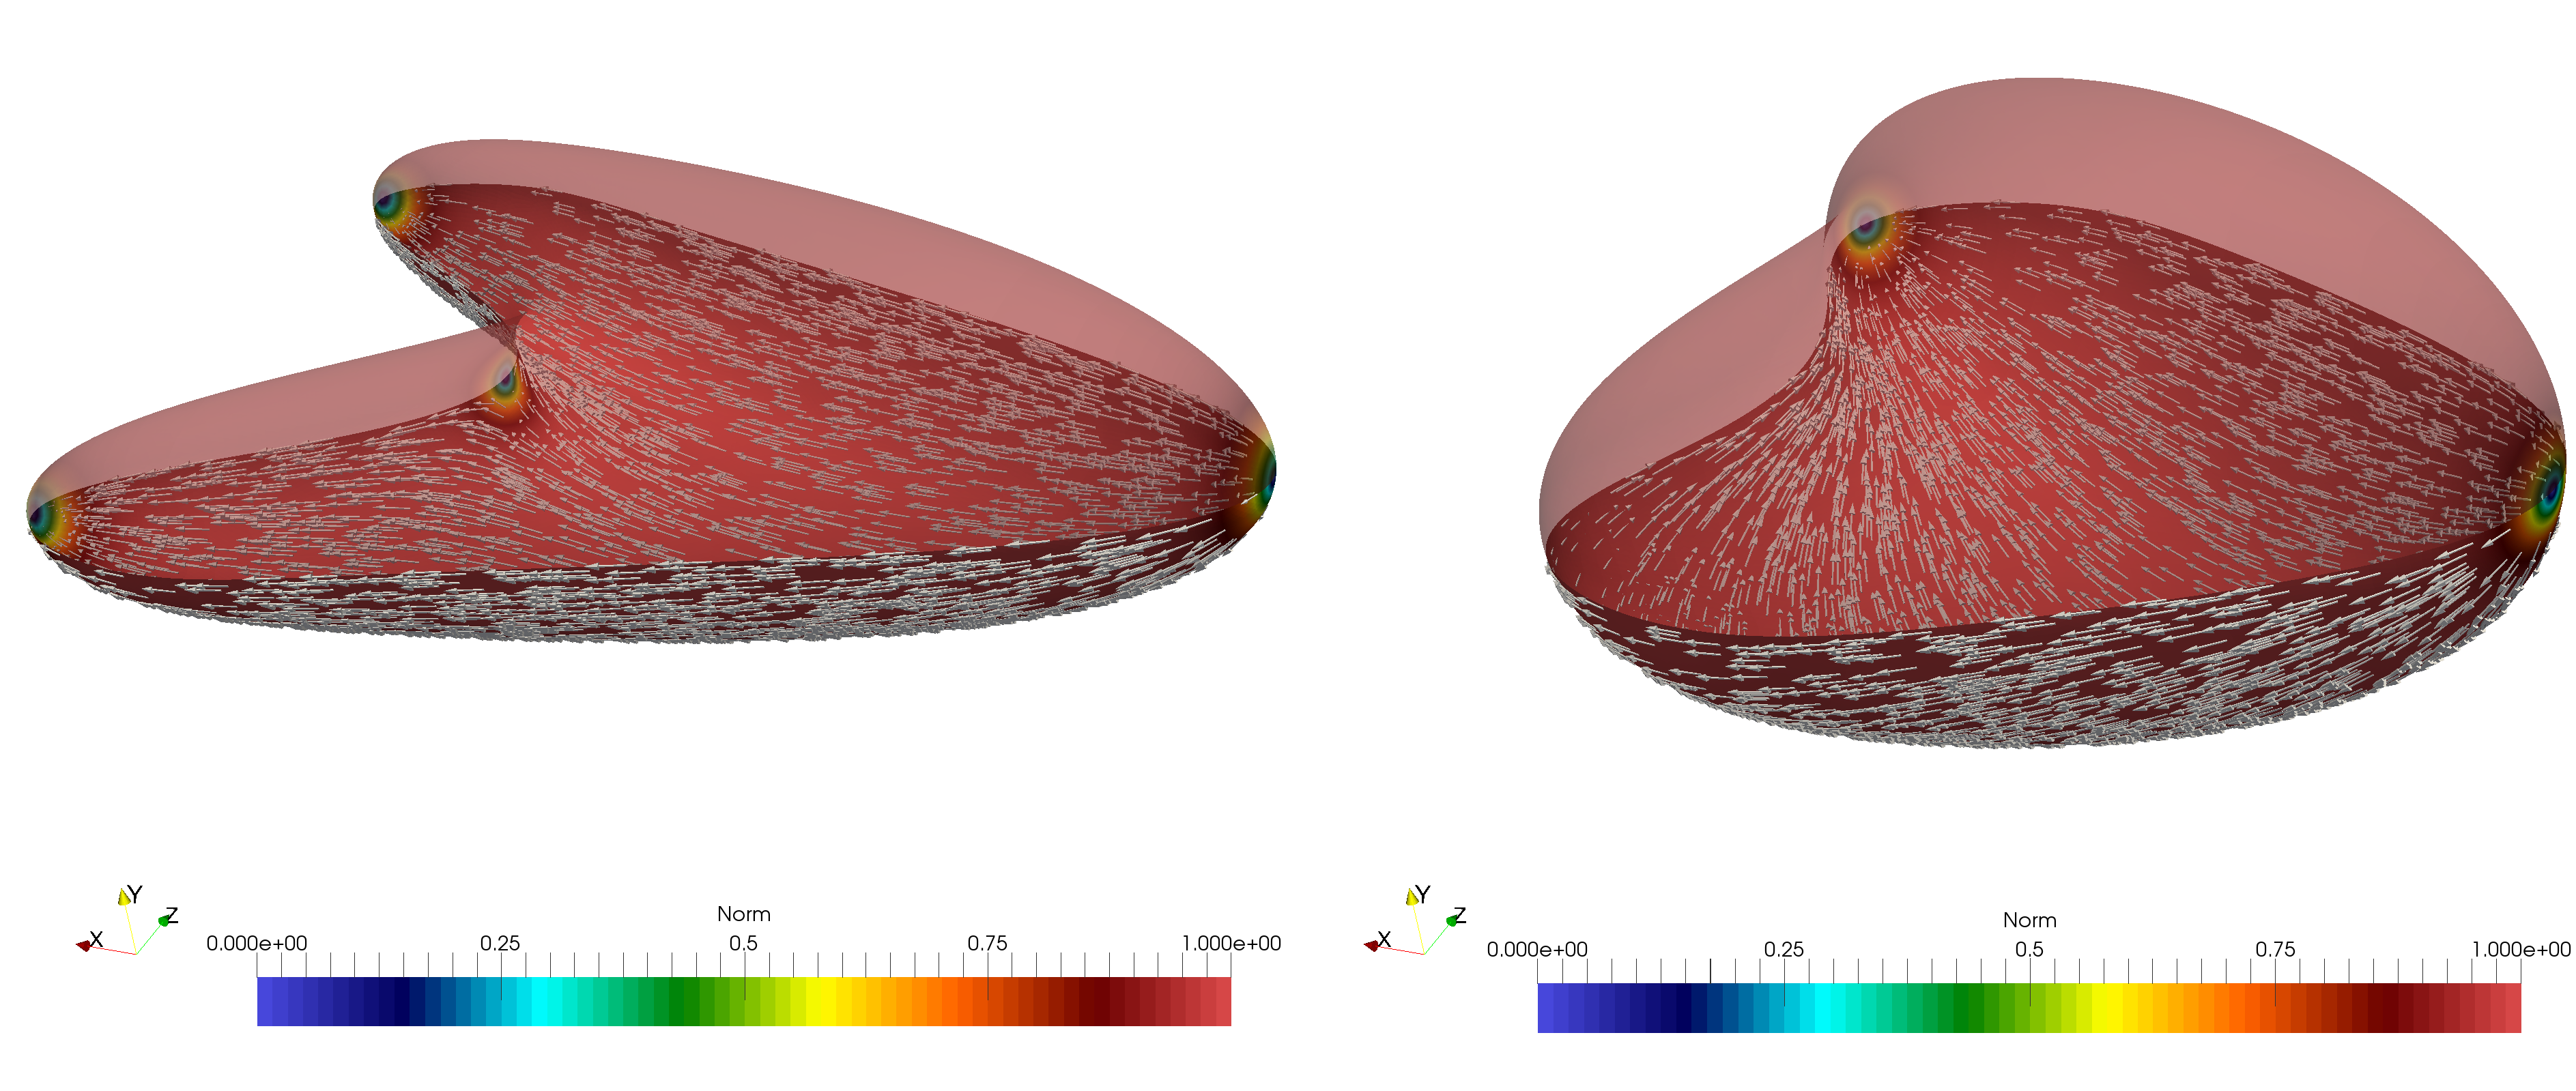
\includegraphics[width=.95\textwidth]{stuff/paraview/NonicFinal4Defects.png}
  \caption{Nonic Surfaces with \( \pprop = 0.95 \). 
            In the left figure (\( \ppress = 0.56 \), \( \pstretch = 1.6 \)) we see a directional field with stable 4 defect configuration.
            In the right figure (\( \ppress = 0.2625 \), \( \pstretch = 0.75 \)) the 4 defect initial configuration was not stable,
            therefor the system was finally gasp to a 2 defect solution.
           }
  \label{fig:NonicFinal4Defects}
\end{figure}
For the initial solution \( \alphab^{0} \) we can use the \( x \)-coordinate potential, \ie,
\begin{align}
  \alphab^{0} = \frac{\exd x}{\left\| \exd x \right\|_{\varepsilon}} \formComma
\end{align}
where
\begin{align}
  \left\| \qb \right\|_{\varepsilon} &=
      \begin{cases}
        \infty & \text{ if } \left\| \qb \right\| < \varepsilon \\
        \left\| \qb \right\| & \text{ else}
      \end{cases}
\end{align}
to prevent ill well-defined in the defect locations. 
In our experiments \( \varepsilon \) is mostly chosen by \( 10^{-10} \).
Hence, the corresponding contravariant vector field is
\begin{align}
  \pb^{0} &= \frac{\Grad x}{\left\| \Grad x \right\|_{\varepsilon}}\formPeriod
\end{align}
With the projection map
\begin{align}
  \ProjectSurf = I - \frac{\nabla\varphi}{\left\| \nabla\varphi \right\|} \otimes \frac{\nabla\varphi}{\left\| \nabla\varphi \right\|}
\end{align}
we can use in euclidean coordinates the identity
\begin{align}
  \Grad x &= \ProjectSurf\nabla x = \ProjectSurf\EuBase{x} \formPeriod
\end{align}

\subsubsection{PD-1-Form Discretization}
We can discretize the exact 1-form \( \exd x \) on an edge \( e=\left[ v_{1} , v_{2} \right]\in\Es \) by (Stokes theorem)
\begin{align}
  \left( \exd x \right)_{h}(e) = v_{2}^{x} - v_{1}^{x} \formPeriod 
\end{align}
If the face \( \face_{1}\succ e \) is right of the edge \( e \) and \( \face_{2}\succ e \) located left, 
so that \( \star e = [c(\face_{1}),c(\face_{2})] \) is the dual edge, than we can approximate
\begin{align}
  \left( *\exd x \right)_{h}(e) &= -\frac{\left| e \right|}{\left| \star e \right|} \left( \exd x \right)_{h}(\star e)
                                 = -\frac{\left| e \right|}{\left| \star e \right|} \left( \left[c(\face_{2})  \right]^{x} - \left[c(\face_{1})  \right]^{x} \right)
\end{align}
With the discrete norm \eqref{eqPDNorm} of PD-1-forms, we obtain the discrete initial PD-1-form on \( e \in \Es \) by
\begin{align}
  \alphav^{0}(e) = \frac{
                   \begin{bmatrix}
                      v_{2}^{x} - v_{1}^{x}\\
        -\frac{\left| e \right|}{\left| \star e \right|} \left( \left[c(\face_{2})  \right]^{x} - \left[c(\face_{1})  \right]^{x} \right)
                   \end{bmatrix}
                }{\sqrt{\frac{1}{\left| e \right|^{2}}\left(v_{2}^{x} - v_{1}^{x}  \right)^{2}
                                 +\frac{1}{\left| \star e \right|^{2}}\left( \left[c(\face_{2})  \right]^{x} - \left[c(\face_{1})
                                 \right]^{x}\right)^{2} }} \formComma
\end{align}
if \( \sqrt{\frac{1}{\left| e \right|^{2}}\left(v_{2}^{x} - v_{1}^{x}  \right)^{2}
                                 +\frac{1}{\left| \star e \right|^{2}}\left( \left[c(\face_{2})  \right]^{x} - \left[c(\face_{1})
                                 \right]^{x}\right)^{2} } \ge \varepsilon \),
else we set \( \alphav^{0}(e) = [0,0]^{T} \).


\subsection{2 Defect Init}
To provoke a 2 defect solution in the equilibrium, like in \autoref{fig:NonicFinal4Defects} (right), 
we use a normalized projected slightly rotated \( \EuBase{y} \) Field, see \eg, \autoref{fig:Init2Defects}.
\begin{figure}
  \centering
  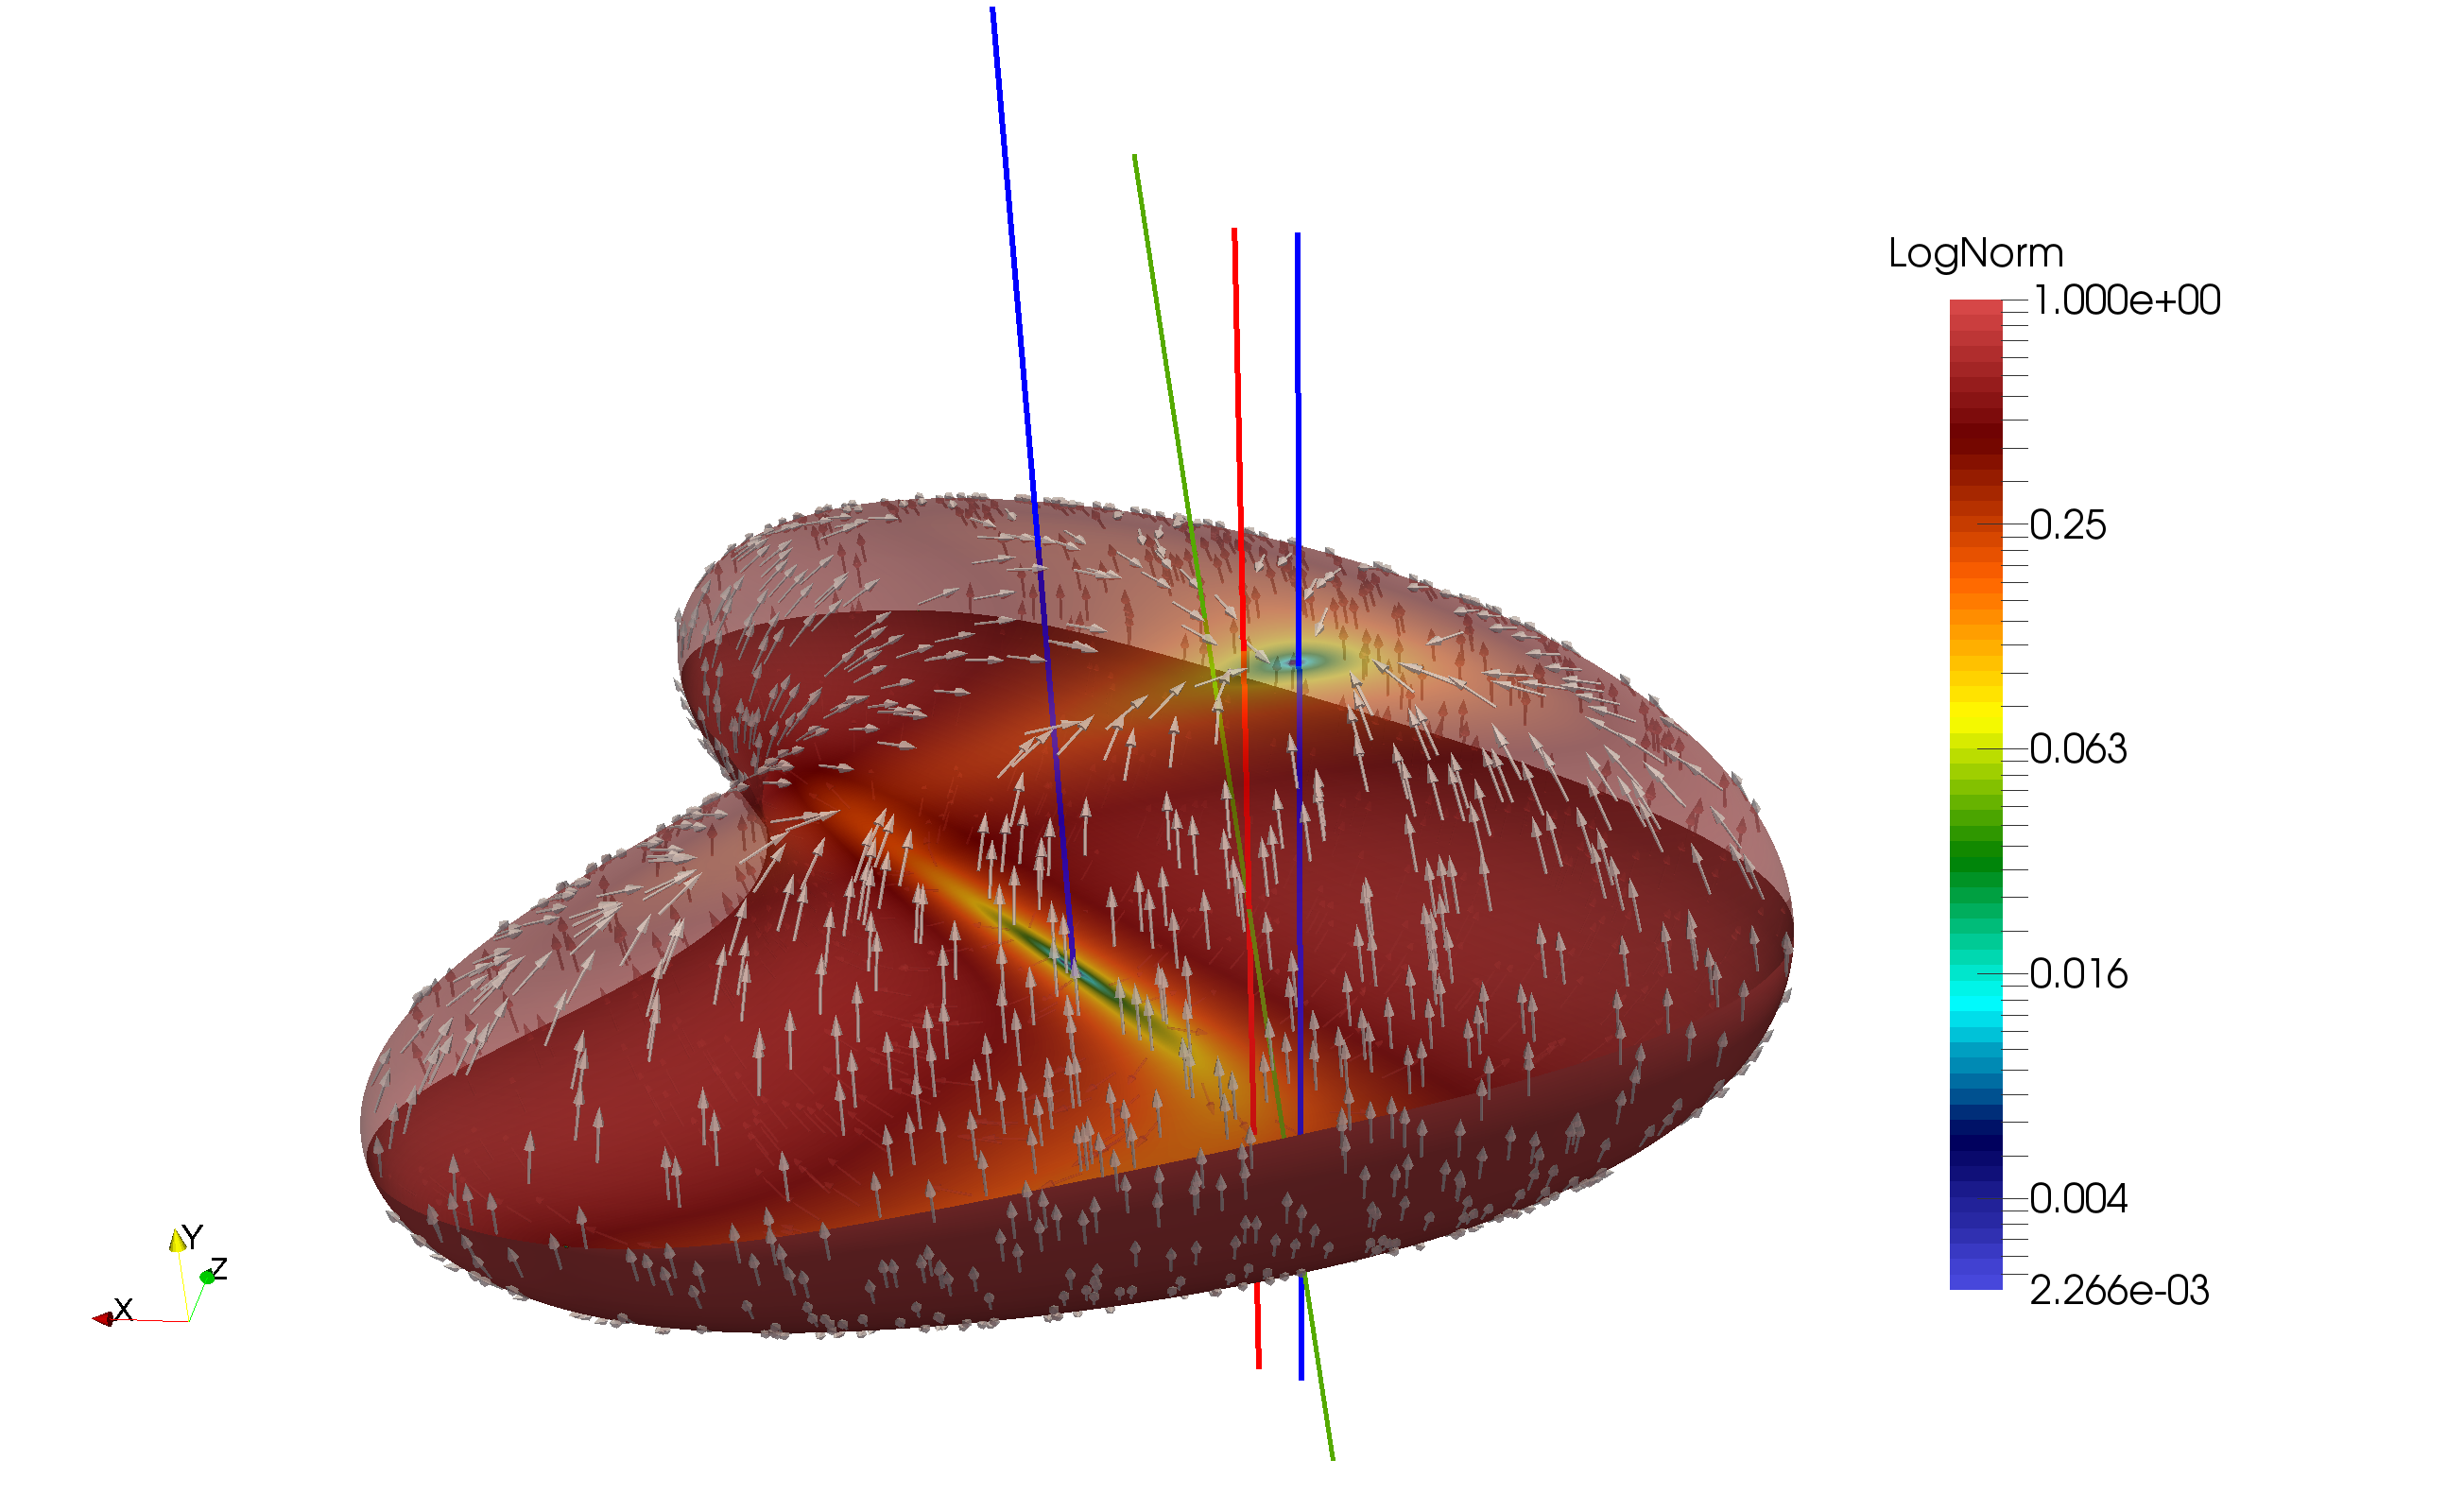
\includegraphics[width=.95\textwidth]{stuff/paraview/Init2Defects.png}
  \caption{Nonic Surface with \( \pprop = 0.95 \), \( \ppress = 0.35 \) and \( \pstretch = 1 \). 
           The green line is the \( y \)-axis and the red line is the rotated \( y \)-axis throw the origin.
           This is a rotation by a radian of \( \gamma = 1.5 \) in the normal plane of the vector 
           \( [-1,0,1]^{T} \).
           The defect locations are at the points, where the rotated \( y \)-axis is orthogonal to the surface (see blue lines).
           The colouring is the logarithm of the norm of the resulting unnormalized vector field \(\check{\pb}^{0}\).
           The arrows show the normalized vector field \(\pb^{0}\).
           }
  \label{fig:Init2Defects}
\end{figure}
With the symmetry of the surface, \( \ProjectSurf\EuBase{y} \) would be result in a metastable state.
To disturb this, we define a rotation \( R_{\gamma}  \) by an angle \( \gamma \) in the normal plane of the vector \( [-1,0,1]^{T} \),
\ie,
\begin{align}
    R_{\gamma} &:=
      \begin{bmatrix}
        \frac{1+\cos\gamma}{2}      & -\frac{\sin\gamma}{\sqrt{2}}  & \frac{-1+\cos\gamma}{2} \\
        \frac{\sin\gamma}{\sqrt{2}} & \cos\gamma                    & \frac{\sin\gamma}{\sqrt{2}} \\
        \frac{-1+\cos\gamma}{2}     & -\frac{\sin\gamma}{\sqrt{2}}  & \frac{1+\cos\gamma}{2}
      \end{bmatrix} \formPeriod
\end{align}
Hence, we get the unnormalized vector field \( \check{\pb}^{0} := \ProjectSurf R_{\gamma} \EuBase{y} \).
The advantage of \( \check{\pb}^{0} \) is that one of the two defects is closer on the larger bulge.
so that the defect move to them in the evolution and not to the smaller bulge.

\section{Appendix}
\subsection{Some Reverse Transformations}
\begin{align}
  \cos\theta &= z\\
  \sin\theta &= \sqrt{1-z^{2}}\\
  \cot\theta &= \frac{z}{ \sqrt{1-z^{2}}}\\
  \csc\theta &= \frac{1}{ \sqrt{1-z^{2}}}\\
  \cos\phi  &= \frac{x-f(z)}{\sqrt{1-z^{2}}}\\
  \sin\phi &= \frac{y}{(1-B)\sqrt{1-z^{2}}}\\
\end{align}



\end{document}
